%\part*{Lezione 19/04/2021}
\section{Metodi indiretti}
Passiamo ora a illustrare 3 metodi di misura indiretti\footnote{Per approfondire Tribble, R.E. et al., Rep.Prog.Phys., 2014, vol.77, \texttt{DOI:}\doi{10.1088/0034-4885/77/10/106901}\articolo{Tribble et al.}.}: \textit{Coulomb dissociation method} (CD), \textit{Trojan Horse method} (TH) e \textit{Asymptotic Normalization Coefficients method} (ANC)

\subsection{\textit{Coulomb Dissociation method}}\index{Coulomb dissociation method@\textit{Coulomb dissociation method}}\label{sec-CD}
$$a+X \to Y+b$$
dove spesso $b\equiv \gamma$. Invece di studiare questa ci concentreremo sulla fotodisintegrazione\index{fotodisintegrazione}:
$$\gamma + Y \to X+ a$$
Dallo studio della sezione d'urto\footnote{Ricordarsi che il fotone ha solo 2 polarizzazioni possibili.}, detta $S$ la matrice di scattering:
\begin{align*}
	\sigma_{aX} &= \frac{\pi}{k_1^2}\frac{1}{(2S_a+1)(2S_X+1)} \: \sum_\ell (2\ell+1) |S_{if}|^2 \\
	\sigma_{\gamma Y} &= \frac{\pi}{k_2^2}\frac{1}{2\,(2S_Y+1)} \: \sum_\ell (2\ell+1) |S_{fi}|^2 
\end{align*}
con $k_1\equiv\sqrt{2\mu_{aX}E_{CM}}$, $k_2\equiv E_\gamma = Q+E_{CM}$\footnote{Abbiamo trascurato il rinculo del nucleo $Y$.} e $S_{if} = (S_{fi})^*$, per cui $|S_{if}|= |S_{fi}|$. Da questo otteniamo il \textbf{principio del bilancio dettagliato}\index{principio del bilancio dettagliato}:
$$\frac{\sigma_{aX}}{\sigma_{\gamma Y}} = \frac{k_2^2}{k_1^2} \frac{2\,(2S_Y+1)}{(2S_a+1)(2S_X+1)}$$
che deriva dall'invarianza per inversione temporale dell'interazione elettromagnetica. Dunque se misuriamo $\sigma_{\gamma Y}$ abbiamo una stima di $\sigma_{aX}$. Sperimentalmente viene fatto interagire $Y$ con una targhetta pesante $Tg$ (tipo piombo) così che la reazione $Y\gamma$ sia dovuta a un fotone virtuale $\gamma^*$. Schema in Figura \ref{0419_schema}.

\begin{figure}[h]
	\centering
	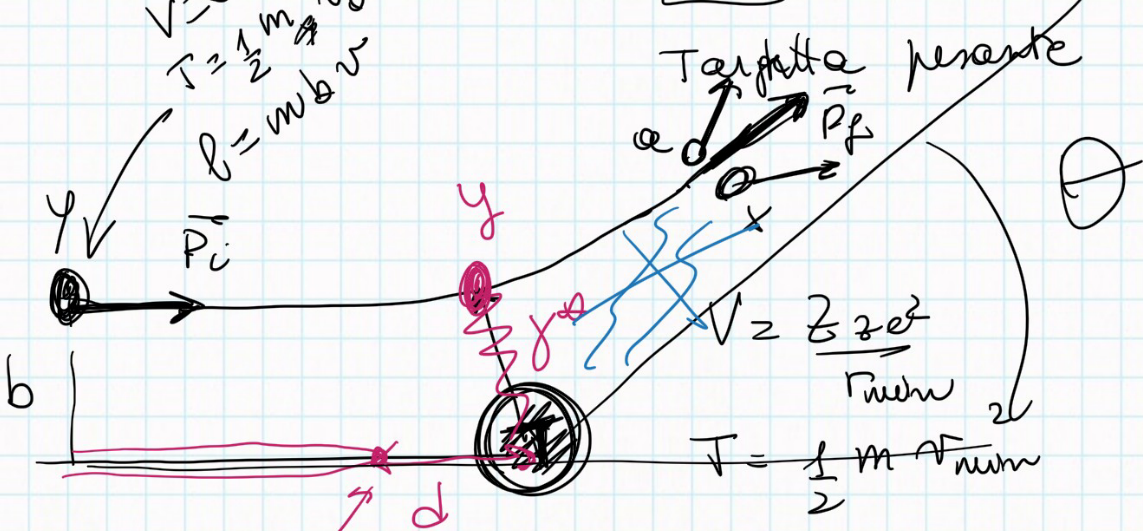
\includegraphics[scale=0.6]{Immagini/0419_schema.png}
	\caption{Schema dello scattering con targhetta pesante. Notazione: $d$ distanza minima se il parametro di impatto è nullo, $b$ parametro di impatto, $\theta$ angolo di scattering.}
	\label{0419_schema}
\end{figure}

\noindent Se il parametro di impatto è nullo, $b=0$, si ha nel punto di minima distanza: $V=Zz e^2 / d$ e $T=0$. Dalla conservazione dell'energia, con $v_0$ velocità iniziale:
$$d= 2\frac{zZe^2}{mv_0^2}$$
In generale: $V=Zz e^2 / r_{\min{}}$, $T=m v_{\min{}}/2$ e $\ell = m r_{\min{}}v_{\min{}}$. Se supponiamo di avere scattering elastico allora $\Delta p\equiv |p_i-p_f| = 2p \sin{(\theta/2)} = 2m v_0 \sin{(\theta/2)}$. Dalla relazione tra variazione di impulso e forza si ha $\Delta p = \int F\, dt = zZ e^2\int \cos{\beta}\: dt/r^2 $, dove $\beta$ è l'angolo formato dalla bisettrice dell'angolo $\pi - \theta$ e il vettore distanza tra $Y$ e $Tg$:  se $Y$ arriva da $-\infty$ a $t=0$ si ha $\beta(0) = - (\pi-\theta)/2$, mentre a $t=\infty$ $\beta(\infty) = (\pi-\theta)/2$.\\
Per trovare la relazione funzionale tra $\beta$ e $t$ scriviamo la conservazione del momento angolare\footnote{$\vec{v}$ in coordinate polari: $\vec{v} = \dot{r}\, \hat{r} + r \dot{\beta}\, \hat{\beta}$}:
$$m v_0 b = m r^2 \dot{\beta} $$
$$\frac{dt}{r^2} = \frac{d\beta}{v_0b}$$
Dunque:
$$2mv_0 \sin{\frac{\theta}{2}} = \frac{zZe^2}{v_0 b} \int_{-\frac{\pi-\theta}{2}}^{+\frac{\pi-\theta}{2}} \cos{\beta} \, d\beta$$
$$b = \frac{d}{2}\, \cot{\frac{\theta}{2}}$$
dove abbiamo usato l'esperessione di $d$ trovata in precedenza.\\
A questo punto come al solito facciamo alcune approssimazioni:
\begin{enumerate}
	\item Trascuriamo l'interazione nucleare (altrimenti non avrei $\gamma$ virtuale), per cui $b\gg1$ e di conseguenza $\theta\ll1$.
	\item Facciamo l'approssimazione \textit{one-photon-exchange}\index{one photon exchange@\textit{one-photon-exchange approximation}}, quindi abbiamo lo scattering con un solo fotone e trascuriamo l'interazione (\textit{photon exchange}) tra i prodotti $a$ e $X$ con il nucleo pesante (\textit{post-acceleration effects}).%%! DA CAPIRE MEGLIO
\end{enumerate}
\noindent Date queste due assunzioni, la velocità relativa tra i prodotti è piccola per cui possiamo lavorare a energie maggiori, migliorando così la rivelazione e risolvendo le difficoltà con la barriera di Coulomb.
$$Y + Tg \to Tg + a + X \quad \Rightarrow \quad \gamma^* + Y \to a + X$$
Dalla misura della prima abbiamo la seconda. Non svolgiamo il calcolo, ma riportiamo il risultato solo per i multipoli elettrici:
$$\frac{d^2\sigma}{d\Omega\, dE_\gamma} = \frac{1}{E_\gamma} \frac{d \sigma_{E\lambda}^\gamma}{dE} \frac{dn_{E\lambda}}{dE}$$ 
dove l'ultima derivata è la densità di $\gamma^*$ nello spazio delle fasi e dipende solamente dalla cinematica, non da $Y$ (quindi possiamo calcolarla). Per quanto riguarda la derivata\footnote{Osserviamo che il fattore moltiplicativo ricorda quello del rate in equazione \eqref{0308_rate} vista per il decadimento $\gamma$, dove però avevamo $\lambda = J$.} della sezione d'urto in funzione dell'energia:
$$\frac{d\sigma_{E\lambda}^\gamma}{dE} \sim \frac{(\lambda +1)}{\lambda[(2\lambda + 1)!!]^2} E_\gamma^{2\lambda -1} \frac{d}{dE}(B(E\lambda))^*$$
dove $B$ è la \textit{reduction transition probability}\index{reduction transition probability@\textit{reduction transition probability}} definita come:
$$B(E\lambda, J_i \to J_f) = \frac{1}{2J_i +1 } \: \pp{|}{\emat{J_f}{\underbrace{Y_{\lambda \mu}(\hat{r}) r^\lambda \rho(\vec{r})}_{E\lambda}}{J_i}}{|}^2$$
L'elemento di matrice di multipolo si può stimare tramite le stime di Weisskopf\index{stime di Weisskopf}\footnote{Vedi \secrif{sec-stime-Weiss}.}.\\
Da $d^2\sigma/d\Omega\,dE_\gamma$ si ottiene $\sigma_{E\lambda}^\gamma$ e da questa $\sigma_\text{cattura}$. Conta in particolare $E1$, ma verificare che il contributo dei termini superiori $\lambda >1$ (per esempio $M1$ ed $E2$) è \vir{piccolo} non è semplice, c'è molta teoria; inoltre, dev'essere trovato un buon bilancio tra $\theta$ e $b$ per rispettare l'approssimazione 1. e al contempo non rendere troppo difficoltosa la misura di $\theta$\footnote{$\theta\to 0$ non è facile da misurare.}, mentre per mantenere l'approssimazione 2. bisogna aumentare l'energia.

\paragraph{Un esempio} Prendiamo la reazione\footnote{Compare nella $pp$III.}:
$$p+\ce{^7Be} \to \ce{^8B}+\gamma$$
Questa è una reazione studiata molto e con varie tecniche, per cui è un ottimo campione per testare un metodo.\\
Procedendo come abbiamo studiato\footnote{Il piombo dev'essere nel fondamentale.}:%! Perché nel fondamentale? Forse per la produzione di fotoni virtuali?
$$\ce{^8B} + \ce{^{28}Pb} \to p +  \ce{^7Be} + \ce{^{28}Pb} \quad \Rightarrow \quad \gamma^* + \ce{^8B} \to p+ \ce{^7Be}$$
Si sono fatti vari esperimenti a energie differenti\footnote{L'unità di misura AMeV indica \textit{tot} MeV per nucleone.}:
\begin{itemize}
	\item 47 AMeV e 52 AMeV, esperimento RIKEN\esperimento{RIKEN} in Giappone. Questa misura era affetta significativamente dal background dovuto ai fotoni di interazione tra prodotti e targhetta (\textit{multi-photon-exchange}\index{multi-photon-exchange@\textit{multi-photon-exchange}}).
	\item 83 AMeV, esperimento MSU\esperimento{MSU} in America. I rivelatori usati in questa misurazione erano a bassa efficienza.
	\item 254 AMeV, esperimento GSI\esperimento{GSI} in Germania. \acc{E} il migliore tra i tre.
\end{itemize}
\noindent Nel caso dell'ultimo esperimento (quello su cui ci concentriamo) fu fatta un'analisi in multipoli (fino a $E2$). In Figura \ref{0419_gsi} riportiamo i risultati ottenuti, mentre in Figura \ref{0419_esp} sono riportati i risultati anche degli altri esperimenti. Notiamo da quest'ultimo grafico che non vi è accordo, ma ciò è dovuto alle difficoltà spiegate precedentemente (tuttora vi è discussione).

\begin{figure}[h]
	\centering
	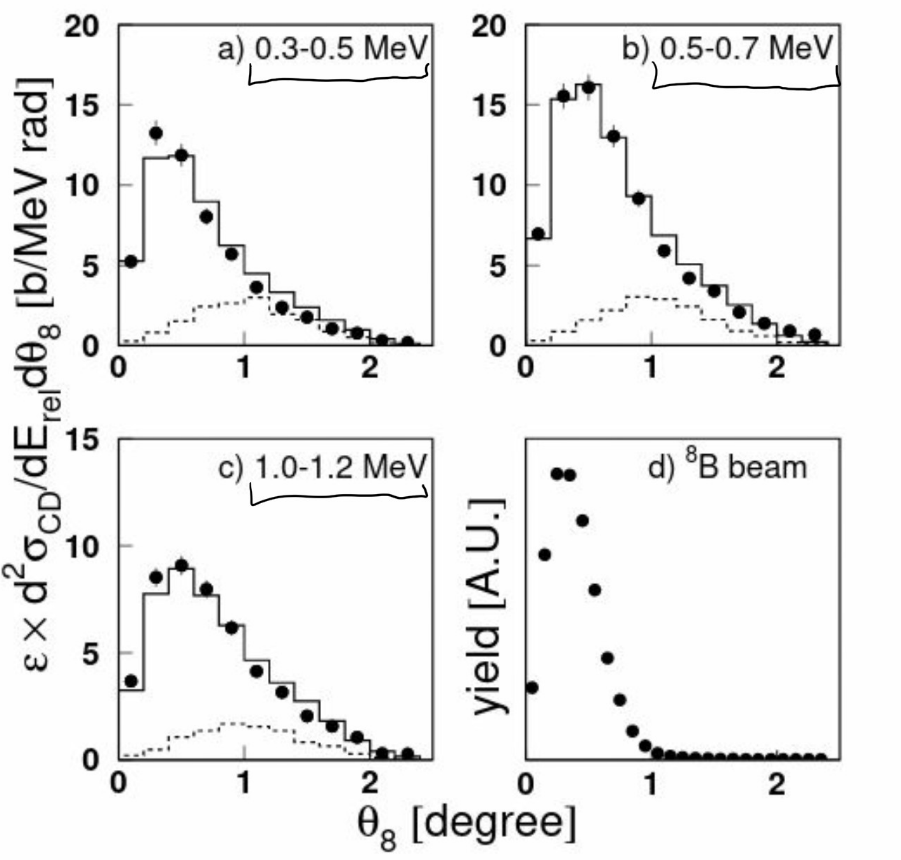
\includegraphics[scale=0.5]{Immagini/0419_ang.png}
	\caption{Risultati dell'esperimento GSI. Il pannello in basso a destra è il fascio di $\ce{^8B}$ che non ci interessa. Negli altri pannelli abbiamo 3 intervalli di energia nel sistema del centro di massa: i punti rappresentano i dati sperimentali, mentre gli istogrammi in linea continua sono simulazioni con il contributo $E1+M1$ e quelli in linea tratteggiata sono simulazioni con il contributo solo di $E2$.}
	\label{0419_gsi}
\end{figure}

\begin{figure}[!h]
	\centering
	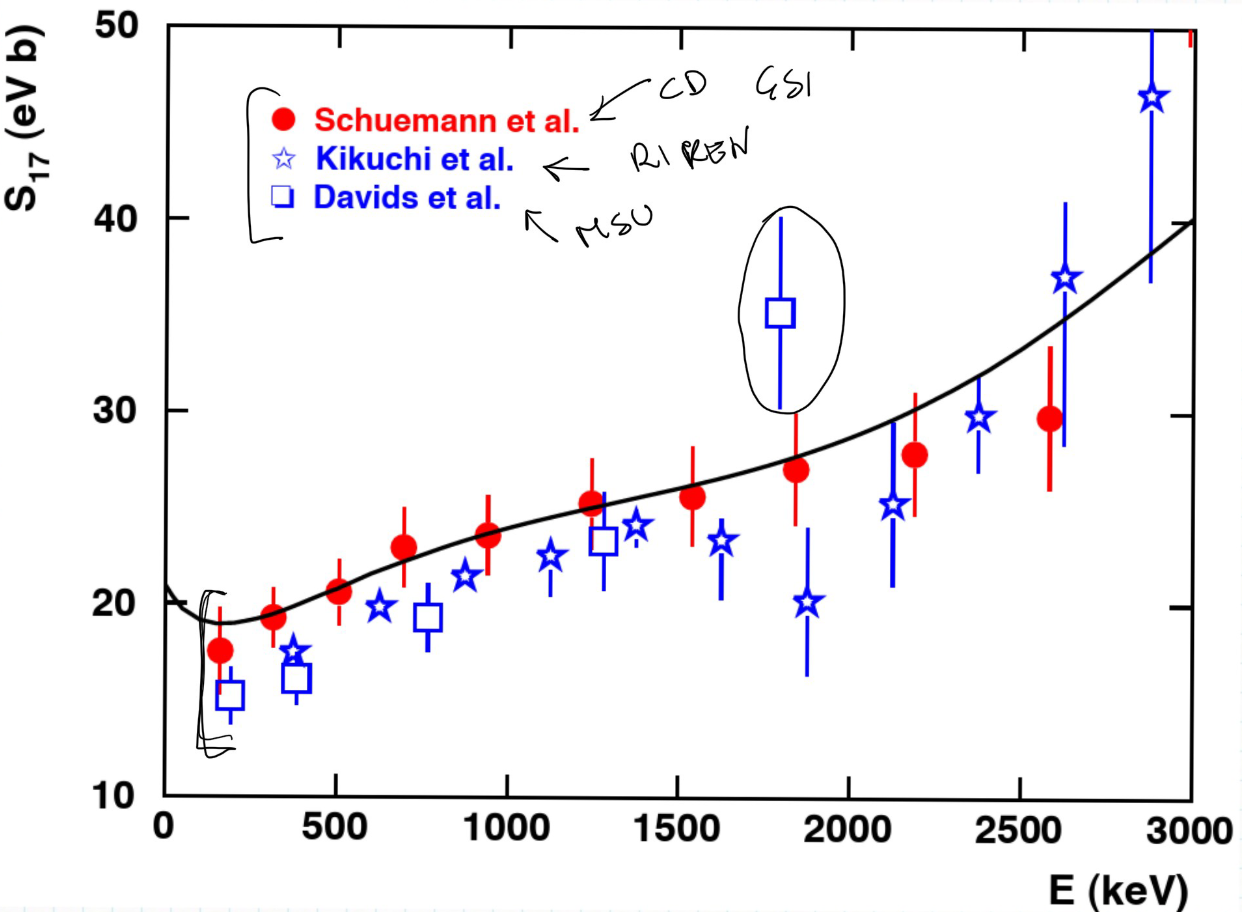
\includegraphics[scale=0.5]{Immagini/0419_Sastr.png}
	\caption{Risultati dei vari esperimenti a confronto.}
	\label{0419_esp}
\end{figure}

\noindent Con questo metodo però non si riescono a vedere le risonanze.

%%!! DI QUESTO PARAGRAFO NON HO CAPITO UNA MAZZA
\paragraph{Un'ultima osservazione} Si può avere $E1$ e $M1$ contemporaneamente, perché lo stato di scattering può avvenire con onde pari o dispari che portano allo stesso $J$, per esempio si potrebbe avere\footnote{Ricordarsi che:%
\begin{align*}
	E&\to\pi=(-1)^L \\
	M&\to\pi=(-1)^{L+1} 
\end{align*}%
} $E1$ in onda $S$ (pari) e $M1$ in onda $P$ (dispari), ma sperimentalmente è impossibile distinguerle; per cui se abbiamo un processo $\gamma + X \to X^* \to a+b$ ($\pi^a=\pi^b=1$) ciò che si vede sono $\sum_\ell (2\ell+1)$ onde, con $\ell$ momento relativo tra i prodotti, quindi non si può distinguere $\ell$.
%!!
\newpage
\subsection{\textit{Trojan Horse method}}\index{Trojan Horse methood@\textit{Trojan Horse method}}\label{sec-THm}
Consideriamo la reazione\footnote{Cambiamo notazione.}:
$$A+x \to C+c$$
L'idea del metodo consiste, come il nome suggerisce, nell'uso di un \vir{cavallo di Troia} per far superare la barriera Coulombiana a $x$: si prende un nucleo $a$ a cluster tale $a=x+b$ dove $b$ è uno spettatore (per rimanere nella metafora fa la parte degli dèi). Avremo allora:
$$A+a \to C+c + b$$
La velocità di $x$ all'interno del nucleo $a$ è vincolata dall'energia di Fermi, quindi nel sistema del laboratorio $\vec{v}_x = \vec{v}_a + \vec{v}_\text{fermi}$; ciò permette di avere alte velocità per $a$ senza però uscire dal range di energie di interesse astrofisico, dato che la velocità relativa tra $x$ e $A$ è limitata. Affinché questa condizione si verifichi, è necessario, però, che il nucleone $b$ si comporti da spettatore, per cui nello studio che faremo ci metteremo nella regione detta quasi-\textit{free}\footnote{In questa regione il momento relativo tra $x$ e $b$ è trascurabile, in altre parole la distanza tra i due nucleoni è massima e l'interazione minima. Si ottiene così che la distanza tra $x$ e $A$ è molto inferiore a quella tra $x$ e $b$.}.

\begin{figure}[ht]
	\centering
	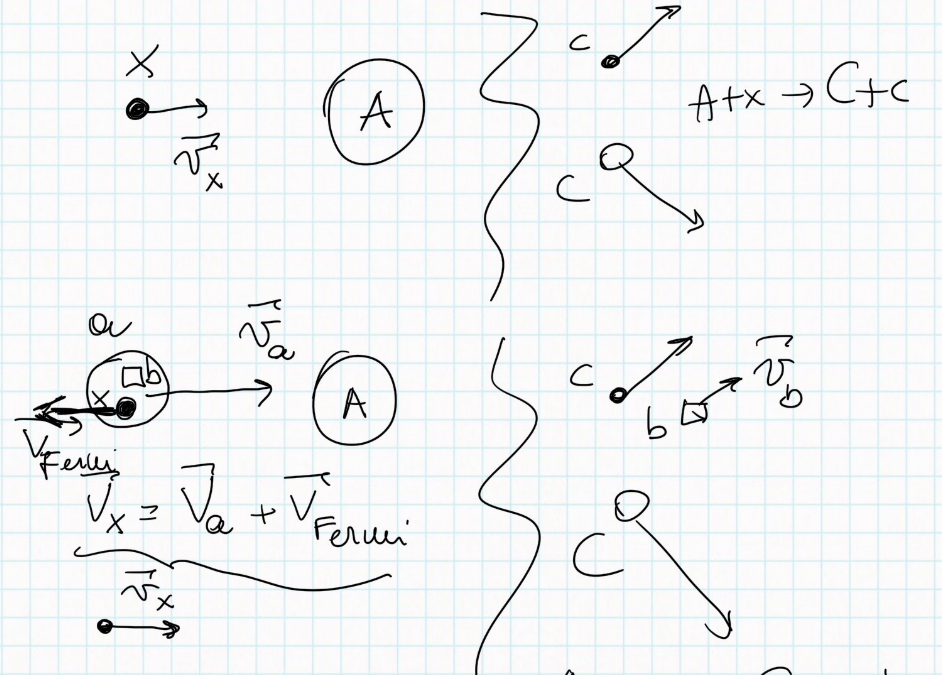
\includegraphics[scale=0.5]{Immagini/0419_scontro.png}
	\caption{Schema della reazione senza THM in alto e con THM in basso.}
	\label{0419_scontro}
\end{figure}

\noindent Questo metodo è stato sviluppato a Catania e anche se coinvolge un processo a 3 corpi in realtà la reazione di interesse è a 2, dal momento che uno di questi è solo uno spettatore. Vediamone gli aspetti principali.

\paragraph{Primi passi} 
Dobbiamo sviluppare una teoria che leghi la sezione d'urto a 3 corpi con quella a 2 corpi. Procediamo per \textit{step}:
\begin{enumerate}[I.]
	\item Lavoriamo in \textit{Distorted Wave Born Approximation}\index{Distorted Wave Born Approximation@\textit{Distorted Wave Born Approximation}}\footnote{In parole povere è come la \textit{Plane Wave Born Approximation} ma si tiene conto di Coulomb.} (DWBA)
	\begin{align*}
		\psi^+(Aa) &\equiv \chi_{Aa}^+\, \phi_A \phi_a \\
		\psi^-(Bb) &\equiv \chi_{Bb}^-\, \psi_{Cc}^- \phi_b
	\end{align*}
	dove $B\equiv C+c$, $\phi$ sono le funzioni d'onda dei vari nuclei, $\chi$ è l'onda distorta e $\psi_{Cc}^- \equiv \chi_{Cc}^-\, \phi_C \phi_c$. Avremo allora che l'elemento di matrice di transizione sarà dato da:
	$$T_{fi} = \oss{\chi_{Bb}^- \psi_{Cc}^- \phi_b}{V_{xb}}{\chi_{Aa}^+\phi_A\phi_a}$$
	$V$ è un operatore interno di $a$.
	\item Poiché $\psi_{Cc}^-$ non è semplice, facciamo la \textit{surface approximation}\index{surface approximation@\textit{surface approximation}}, ovvero approssimiamo la funzione d'onda con il suo andamento asintotico fuori da $R\sim R_{xA}$ (distanza tra i nucleoni), detto per questo \textit{cutoff radius}\index{cutoff radius@\textit{cutoff radius}}; questo ci permette di legare l'elemento di matrice $T_{fi}$ con la $S$-Matrix della reazione a 2 corpi (e quindi allo sfasamento).
	\item Osserviamo che usare la PWBA rispetto alla DWBA influisce solo su un fattore moltiplicativo di normalizzazione dei dati\footnote{Vedi \secrif{compl-dwba-pwba}}. Avremo quindi un fattore astrofisico $S_{TH}(E)$ da riscalare.
	$$\frac{d^3\sigma}{dE_c d\Omega_cd\Omega_{C}} = {K_F}\, \frac{v_{Cc}}{v_{Ax}}\, \pp{|}{W(\vec{P}_{bx})}{|}^2\, \frac{d\sigma^{TH}}{d\Omega_{Ax}}$$ %! Lei scrive a denominatore d\Omega_{-c} ma nell'articolo è scritto così, che vuol di' -c?
	dove $K_F$ è un coefficiente cinematico, le velocità sono quelle relative e $W$ è la \textit{momentum amplitude}, ovvero la distribuzione dei momenti di $x$ in $a$; l'ultimo termine è quello di interesse.
\end{enumerate}
\noindent Il metodo dipende quindi fortemente dalla scelta di $a$ e in Figura \ref{0419_tab} abbiamo riportato alcune configurazioni. Tra questi i migliori sono $d$ e $\ce{^6Li}$.

\begin{figure}[h]
	\centering
	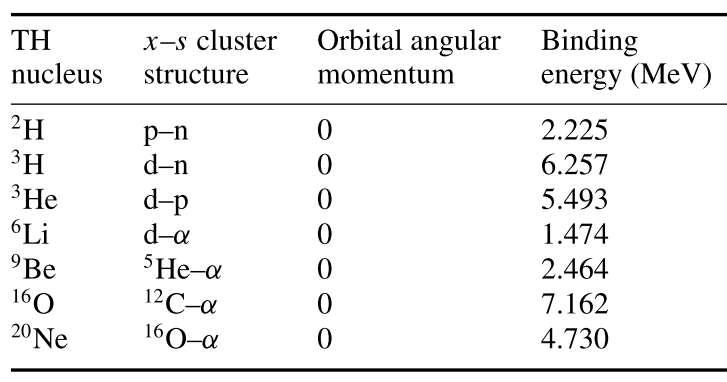
\includegraphics[scale=0.5]{Immagini/0419_tabella.png}
	\caption{Varie possibilità per il nucleo a cluster $a$.}
	\label{0419_tab}
\end{figure}
\newpage
\noindent I criteri per determinare un buon \vir{cavallo} sono:
\begin{enumerate}[(i)]
	\item un'energia di legame $B$ \vir{piccola} nel sistema $x-b$.
	\item una struttura semplice.
	\item un \vir{buon} $Q$-valore per la reazione $A+a\to C+c+b$.
	\item una \textit{momentum amplitude} nota.
	\item una struttura tale da minimizzare i processi non-quasi-\textit{free}, ovvero in cui $b$ non è spettatore.
\end{enumerate}